\chapter{Experimental Evaluation}
\label{chapter:eval}

This chapter describes the testing process of the various components that compose the system architecture. It mostly covers functional testing, but also includes some performance metrics.

\section{Functionality}
\label{sec:func-eval}

\subsection{EFS Tools and EFS Server Tests}
\label{sub-sec:efs-tools-server-tests-eval}

The first level that was tested is the middleware layer presented in \labelindexref{Section}{sec:arch-multi-user}. There are three types of tests that were used for this component.

The first tests the functionality of the C library (EFS Tools). The majority of the tests are Unit Tests which check the functionality of each storage operation available. Additional tests are also used to ensure storage consistency.

An example of a test function is listed in \labelindexref{Listing}{lst:change-passwd-eval}. The \texttt{change_passwd} function tests whether changing the password of the storage works as expected.

\begin{lstlisting}[language=bash, basicstyle=\small, caption=change_passwd test function, label=lst:change-passwd-eval]
function change_passwd() {
    test='Change container password '$1
    #cleaning the logcat again
    adb logcat -c
    adb shell efs-tools storage change_passwd $1 $2 $3
    if [[ `expr length $3` -le "3" ]]; then
        ok0=$(adb logcat -d >  $logfolder/log_change_passwd.log && grep -c 'New passwd too short' $logfolder/log_change_passwd.log)
        if [[ $ok0 == "1" ]]; then
            echo -e "$test did not succeed - password is too short - PASS"
        else
            echo -e "$test did not succeed - password is too short - FAIL"
        fi

    else
        #verify logcat
        ok1=$(adb logcat -d >  $logfolder/log_change_passwd.log && grep -c 'Change passwd successful for '$1' storage' $logfolder/log_change_passwd.log)
        if [[ $ok1 == "1" ]]; then
            echo -e "$test from: $2 to: $3 - PASS"
        else
            echo -e "$test from: $2 to: $3 - FAIL"
        fi
    fi
    adb logcat -c
}
\end{lstlisting}

Note that being a unit test, it only checks if the password is too short, and, if not, whether the change has occurred. In order to verify that the new password is being used, the storage lock and unlock tests must be run using the new password.

In the above, \textit{adb} is the Android Debug Bridge\abbrev{adb}{Android Debug Bridge}, a command line tool used for communicating with an Android device connected through an USB port or with an emulator. \textit{adb logcat} outputs the system log, where the Android system and all applications post log messages. \textit{adb shell [command]} issues a shell command to the device.

The tests were written in a bash script because of the simplicity of starting other processes.

The second type of tests are similar to the aforementioned. The difference is that these tests issue the commands through the EFS Server. In order to do so, a small executable called \textit{edc} is used. This tool is responsible for transforming a command into the format expected by the native service. The \textit{edc} utility is written in C, while the tests themselves are written once again in bash.

The third and final type of test for this component is a stress test. It is actually closer to testing the kernel layer component. The way it operates is it creates a directory hierarchy in a normal location in the file system and a mirrored one in a secure storage. The files in the hierarchy have various sizes and access permissions and soft links are also added. At the end of this process, the resulting directory structures are compared to ensure that the storage functions properly.

Due to the necessity of recursive functions when creating the directory structure, Python has been chosen for this test.

All the test that were run passed, ensuring that the middleware layer provides adequate functionality.

\subsection{EFS Service Tests}
\label{sub-sec:efs-service-tests-eval}

The EFS Service exposes the storage operations to the upper level of the Android system. In order to test the correct functioning of the service, a test application has been written. Similarly to the tests for the middleware layer, the application runs a number of unit tests and a few consistency tests to ensure proper functioning of the EFS Service.

The application was written, as any Android application, in Java. Because of this, mechanisms like objected-oriented programming inheritance can be used to make adding new tests simple. \labelindexref{Listing}{lst:tester-eval} illustrates this. \textit{ms} is the service interface, through which the calls to the C library are made. \texttt{Tester} is the abstract class all classes used for testing must be derived from.

\begin{lstlisting}[language=Java, caption=Tester class, label=lst:tester-eval]
private IEFSService ms;

private abstract class Tester {
    public boolean test() {
        return true;
    }
}
\end{lstlisting}

Adding a new test implies writing a new test class, then adding an instance of the class and a \texttt{TextView} object to a map structure. The \texttt{TextView} should contain the name of the test. It is used to mark the success/failure of the test through its color.

The tests are run as shown in \labelindexref{Listing}{lst:run-eval}.

\begin{lstlisting}[language=Java, numbers=none, caption=EFS Service tests, label=lst:run-eval]
for (Map.Entry<Tester, TextView> en : test2view.entrySet()) {
    en.getValue().setTextColor(en.getKey().test() ? Color.GREEN : Color.RED);
}
\end{lstlisting}

\subsection{User Interface and Applications}
\label{sub-sec:interf-apps-eval}

For the user interface and interaction part, automatic testing is more difficult. Therefore, the tests for user experience were done manually.

As mentioned in \labelindexref{Section}{sub-sec:user-switch-multi-user}, an issue appeared where some applications would crash because of attempts to access the user's data before it was unlocked. This issue has been fixed. However, testing was done only for applications present in the AOSP sources. No third-party applications have been tested and the existence of access patterns that could result in crashes is a possibility.

Applications have been tested in order to ensure that user data is properly preserved after the storage is locked and unlocked again. As with the issue above, only applications from the AOSP sources have been tested in this regard. Other applications could present some issues when storage operations are performed.

Overall, the user should not notice any significant difference between using the same device with or without the multi-user encryption features present. The Quality of Experience is not affected.

\section{Performance}
\label{sec:perf-eval}

For performance testing, the \textit{Bonnie++}\footnote{\url{http://www.googlux.com/bonnie.html}} tool was used. It is a tool designed to test filesystem performance. It runs a variety of tests for reading and writing of files. One of the types of tests attempt to mimic the access pattern that regular applications have in order to provide an accurate measurement of performance. The second type of tests creates and deletes multiple small files in rapid succession.

For the purpose of this project, the tool was first used on a regular location in the filesystem and then on a location where an encrypted storage was mounted. The per character tests have been skipped in favour of the per block ones. The average values resulted from multiple iterations of the tests are shown in \labelindexref{Table}{tbl:res-unenc-eval} for the unencrypted location and in \labelindexref{Table}{tbl:res-enc-eval} for the encrypted storage. The tables have been split in two lines for readability purposes.

It is worth noting that although some of the results are measured in microseconds, the granularity of some tests is not a microsecond, but more close to a millisecond. The reason the values seem to have precision of a microsecond is that the values are the result of averaging the output of multiple iterations of the test.
\newpage

What also stands out is that there is not a significant difference between the two sets of values. This is because, as has been mentioned, \textit{Bonnie++} runs tests that simulate the activity of an actual application, rather than testing the disk or file system for its maximum performance. For measuring usability, this method of testing renders more realistic results.

\begin{table}[ht]
\centering
    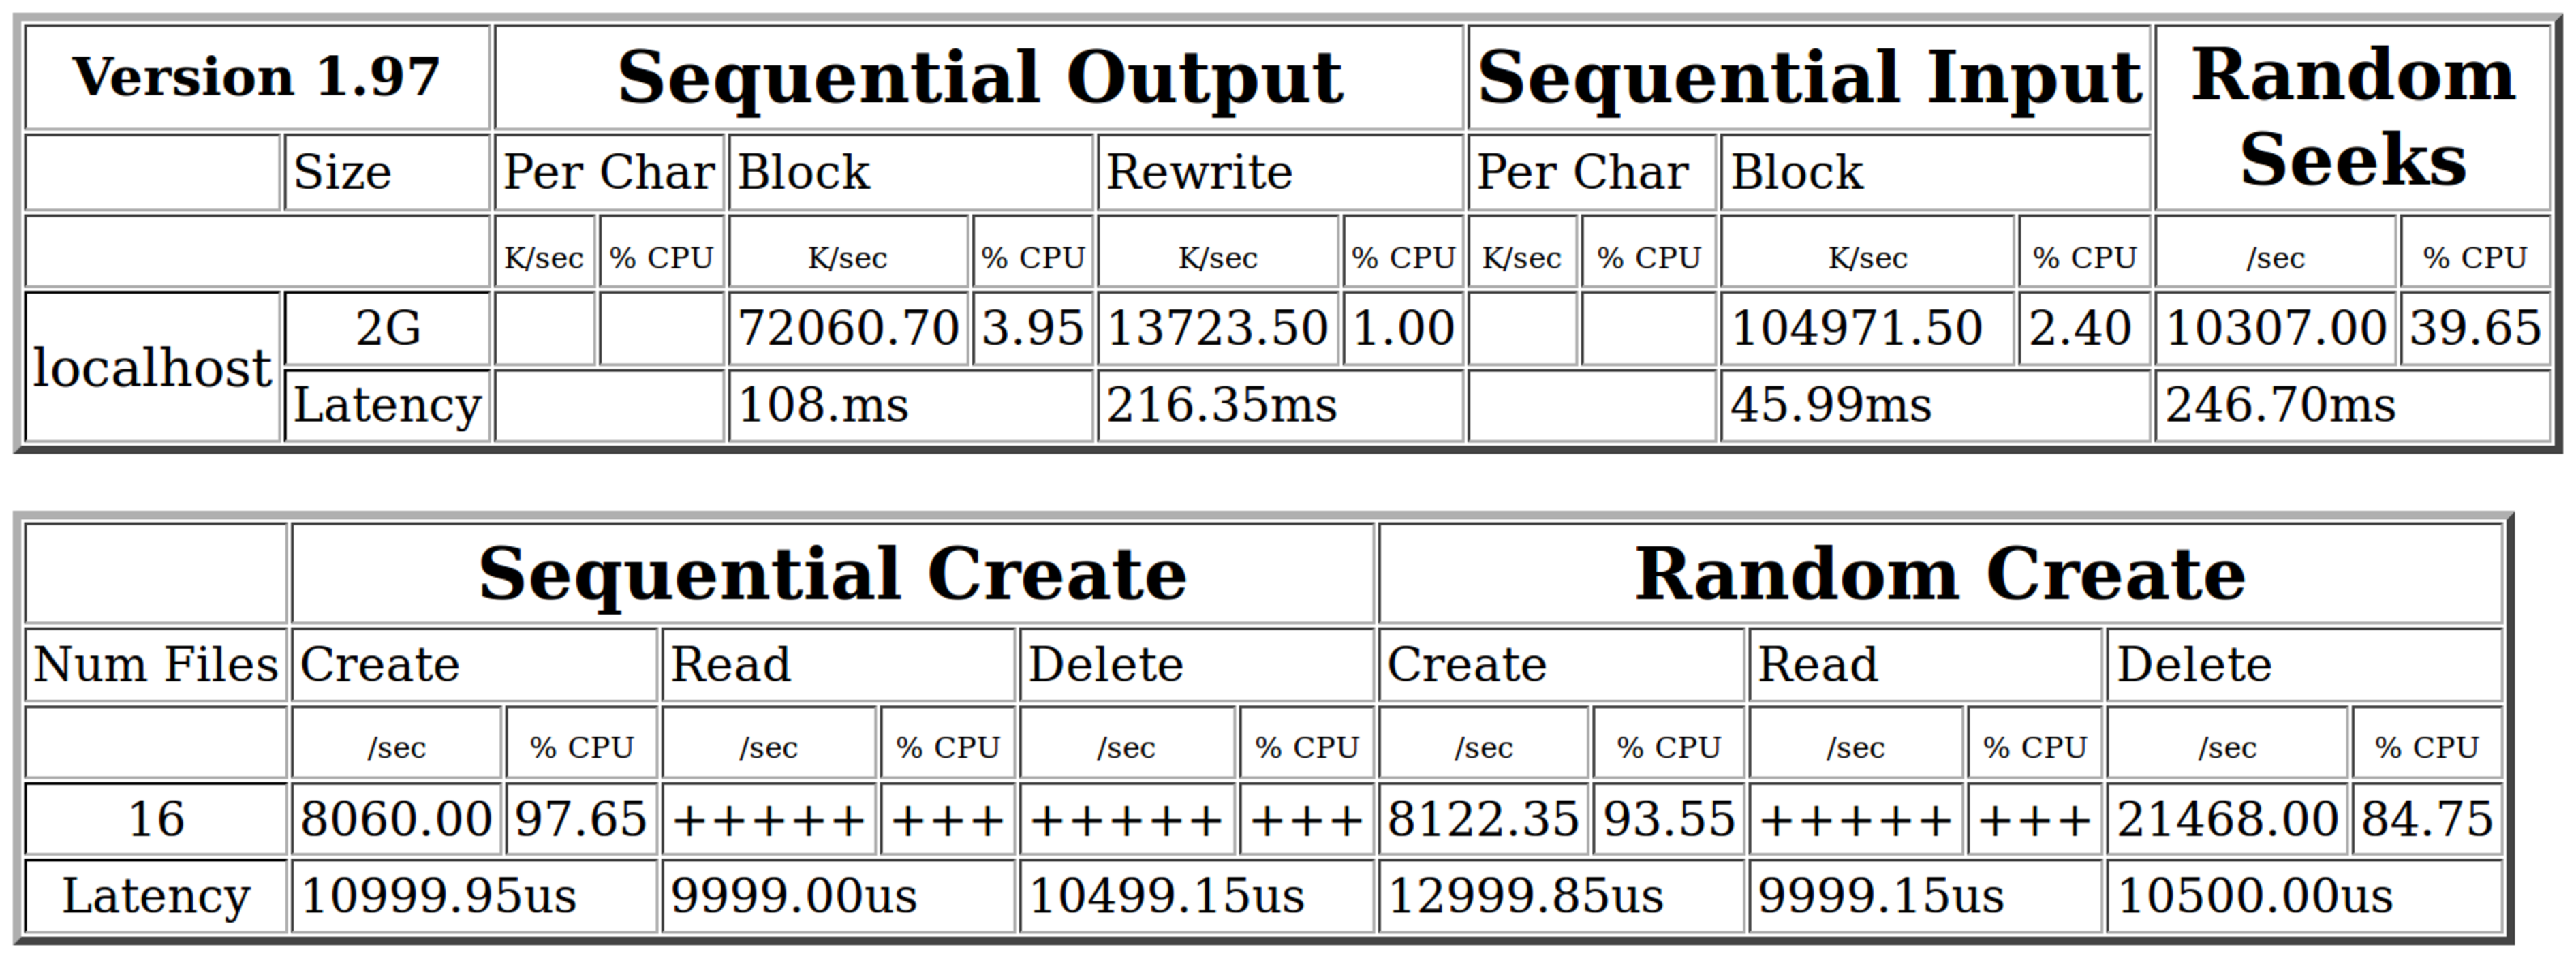
\includegraphics[width=\textwidth]{src/img/perf/results.pdf}
\caption{Bonnie++ results - Unencrypted}
\label{tbl:res-unenc-eval}
\end{table}

\begin{table}[ht]
\centering
    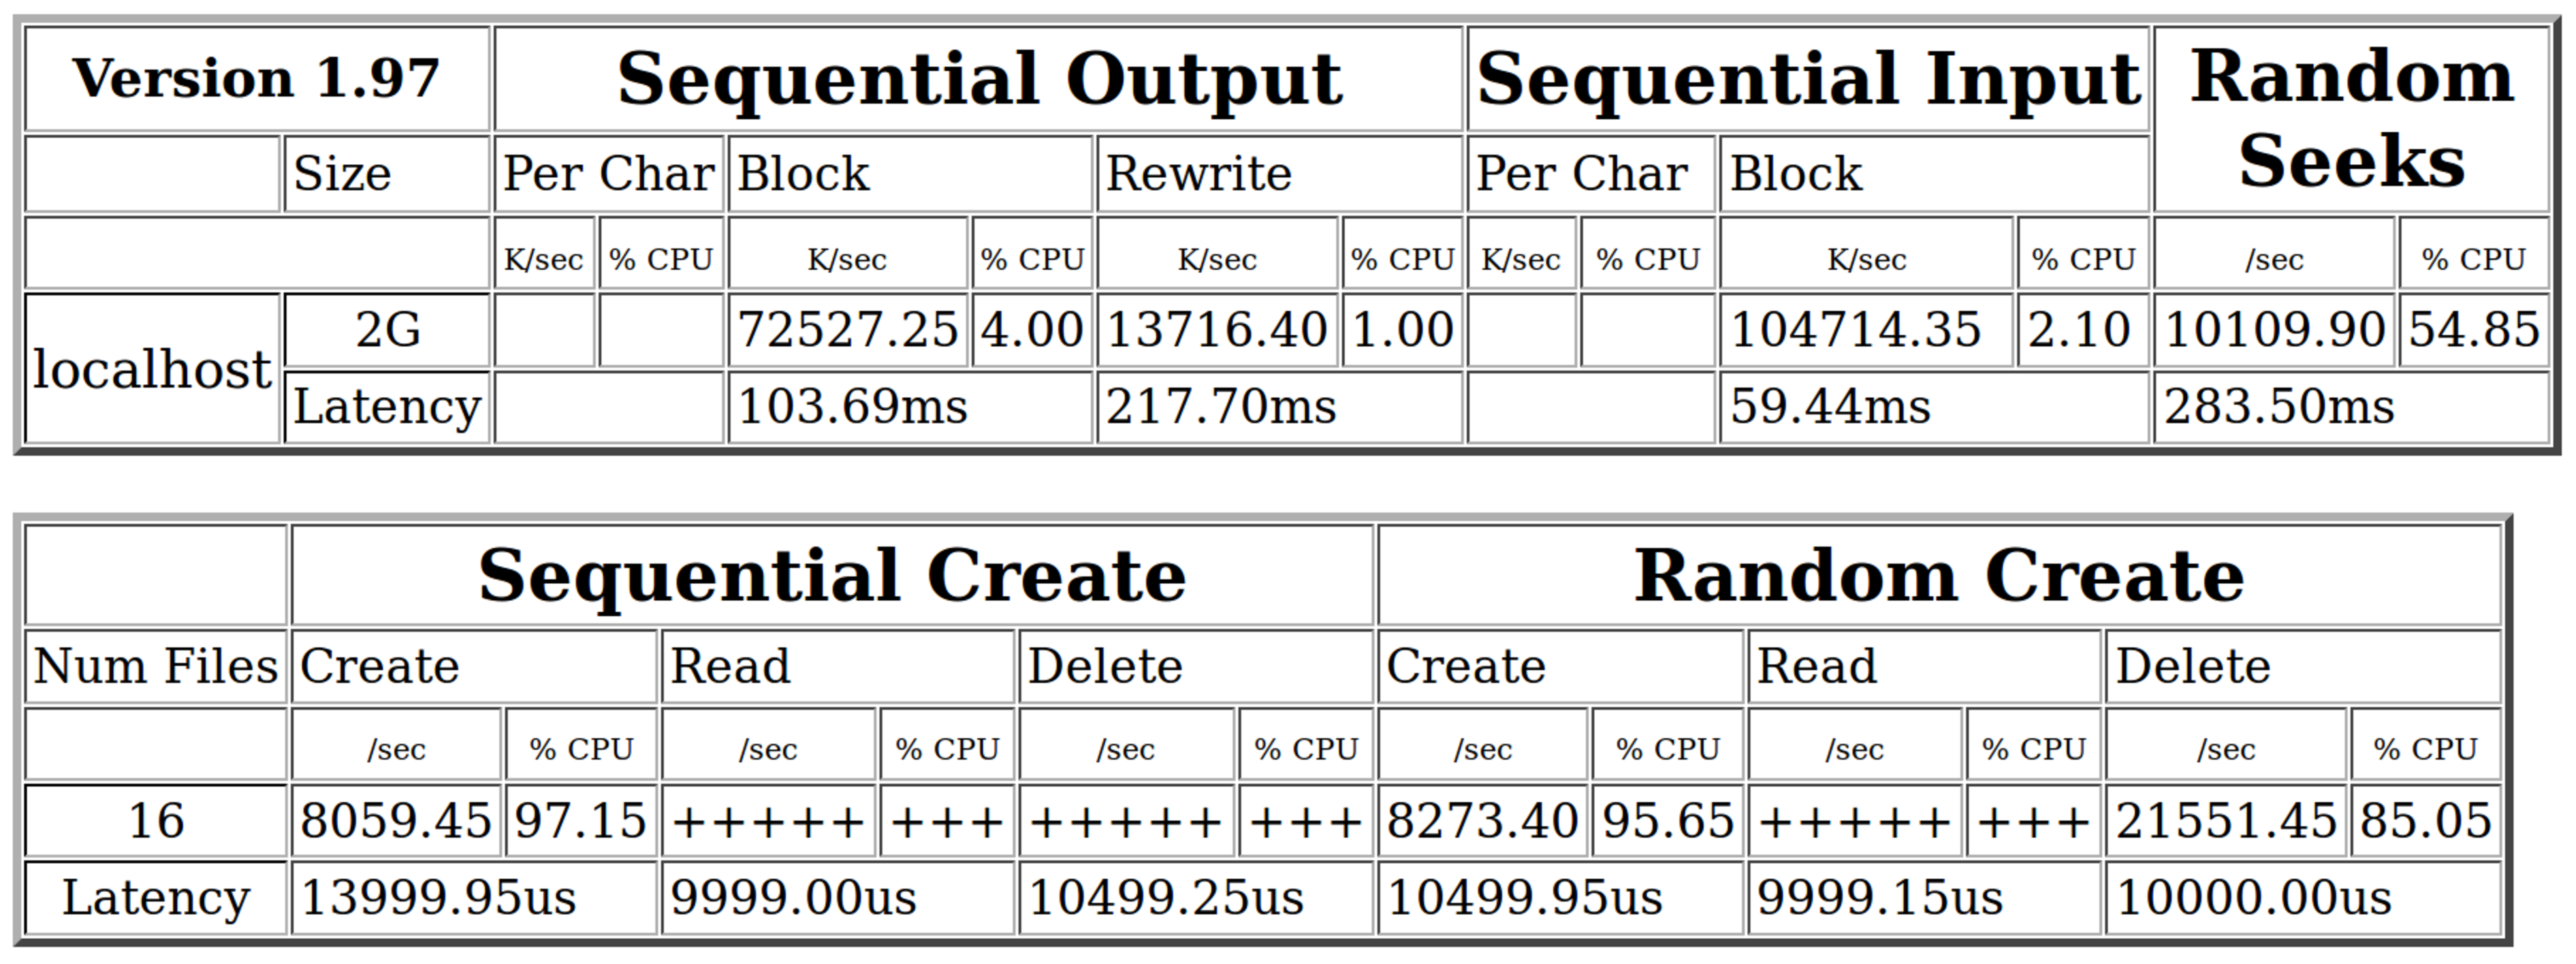
\includegraphics[width=\textwidth]{src/img/perf/results2.pdf}
\caption{Bonnie++ results - Encrypted}
\label{tbl:res-enc-eval}
\end{table}

The conclusion to be drawn from this is that, under regular usage conditions, the difference between a device with multi-user encryption integrated and one without it is not noticeable, especially from the user's point of view.
